\subsection{Harmonic Transition State Theory}
\label{sec:htst}
%\tred{This section is probably missing some citations.}
%
To actually calculate the partition functions can be a tedious task and finding a good transition state is a non-trivial one, if possible (see for example~\cite{ts-opt-2001}).
Fortunately, for many systems (e.g. solid state materials), the transition state can be approximated and the configuration integrals simplified.

\begin{figure}[h]
\begin{center}
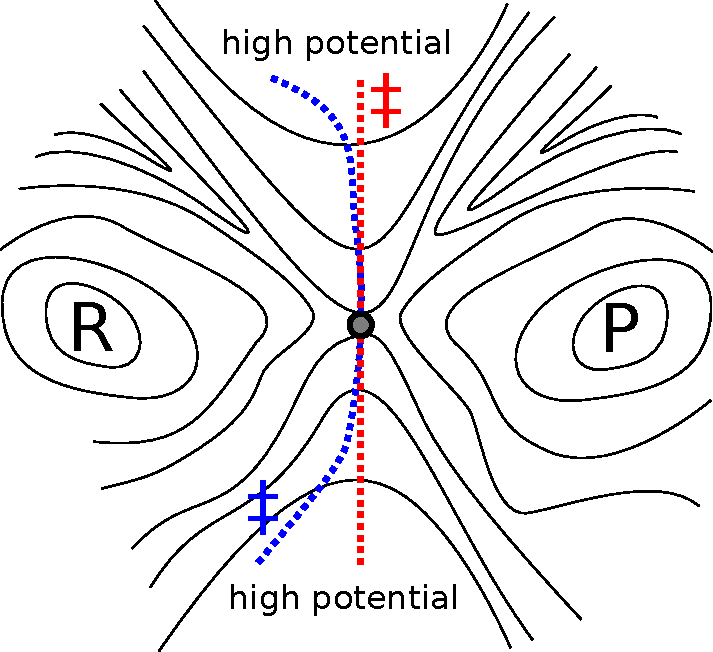
\includegraphics[width=0.5\linewidth]{harmonic-transition-state}
    \parbox{0.85\linewidth}{
\caption{The transition state, (blue $\ts$), and the harmonic transition state (red $\ts$).
The grey circle is a \sap{1}.
}
\label{fig:transition-state}
    }
\end{center}
\end{figure}

Between any two basins there exists a \sap{1}, which represents the lowest possible potential energy that the system must overcome in order for a transition to occur.
Exploiting this, the $\ts$ can be chosen as a hyperplane in which the \sap{1} resides and whose normal is the eigenmode that corresponds with the lowest eigenvalue of the Hessian.
This greatly simplifies the definition of the $\ts$.
Furthermore, in order to simplify the calculation of the partition functions, the PES near both $\ts$, $E_\ts$, and R, $E_\text{R}$, are represented by second degree Taylor expansions,
\beq{htst-taylor-expansion-min}
E_\text{R}(\vect{q}_\text{R}) \approx E(\vR_\text{min}) + \frac{1}{2} \sum_i^{3N} k_{\text{R},i} q_{\text{R},i}^2,
\eeq
\beq{htst-taylor-expansion-sp}
E_\ts(\vect{q}_\ts) \approx E(\vR_\text{\sap{1}}) + \frac{1}{2} \sum_i^{3N-1} k_{\ts,i} q_{\ts,i}^2,
\eeq
where $\vect{q}_{[\ts, \text{R}]}$ are the eigenvectors of the Hessian, $q_{[\ts, \text{R}],i}$ is the displacement along eigenvector $i$, $k_{[\ts, \text{R}],i}$ are the corresponding Taylor coefficients, all for the $\ts$ and R respectively, and $E(\vR_{[\sap{1}, \text{min}]})$ are the energies at the \sap{1} and the minimum of the R basin, respectively.
Since the central points of the expansions are stationary, the first derivatives vanish from the expression, leaving only constants along with the second order terms.

Due to the format of the energy approximations, the configurational integrals become trivial Gaussian integrals,
\beq{htst-gaussian-integral}
\int_{-\infty}^\infty e^{-k_iq_i^2/2 \kB T} dq_i = \sqrt{\frac{2 \pi \kB T}{k_i}}.
\eeq
The reaction rate then reduces to
\beq{htst-reaction-rate-raw}
k_\text{HTST} = \sqrt{\frac{\kB T}{2 \pi \mu}}\frac{e^{-E(\vR_{\sap{1}})/\kB T}\prod_i^{3N-1}\sqrt{\frac{2 \pi \kB T}{k_{\ts, i}}}}{e^{-E(\vR_\text{min})/\kB T}\prod_i^{3N}\sqrt{\frac{2 \pi \kB T}{k_{\text{min}, i}}}}.
\eeq
Most of the $\kB T$ and $2\pi$ parameters cancel each other, leaving only one set by means of the different dimensionality of $\ts$ and R.
Rearrangement of \fref{eq:htst-reaction-rate-raw}, along with the multiplication of $\mu^{3N}$ on both sides of the fraction, yields,
\beq{htst-reaction-rate-cleaned}
k_\text{HTST} = (2\pi)^{-1} \frac{\prod_i^{3N} \sqrt{\frac{k_{\text{min},i}}{\mu}}}{\prod_i^{3N-1} \sqrt{\frac{k_{\ts,i}}{\mu}}}
e^{-(E(\vR_{\sap{1}}) - E(\vR_\text{min})) /\kB T}.
\eeq
Now it is possible to insert the respective vibrational frequencies,
\beq{htst-vibrational-frequencies}
\nu_\text{*} = \sqrt{\frac{k_\text{*}}{\mu}}(2\pi)^{-1},
\eeq
into \fref{eq:htst-reaction-rate-cleaned},
\beq{htst-reaction-rate}
k_\text{HTST} = \frac{\prod_i^{3N}\nu_{\text{min},i}}{\prod_i^{3N-1}\nu_{\ts,i}}
e^{-(E(\vR_{\sap{1}}) - E(\vR_\text{min})) /\kB T},
\eeq
for a rate that depends only on the vibrational frequencies and energies at the \sap{1} and minimum as well as the temperature.
This form of the rate agrees with the empirically observed temperature dependence of the rate originally expressed by Arrhenius~\cite{vant-hoff-1884, arrhenius-1889}.
The potential energy barrier is addressed in the exponent while the entropical effects are addressed in the so-called prefactor.

%\subsubsection{Terminology}
%All the information needed to form a reaction rate within the harmonic approximation to TST is encoded in/near the minimum and \sap{1}.
%This along with the popularity of HTST, has lead to an unfortunate interchangeable use of the terms "transition state" and "saddle point" in the literature.
%Even though the distinction is not overly important within HTST, it is of central importance in TST, as the actual definition of the transition state is vital.
